\documentclass[serif,aspectratio=169]{beamer}
\usepackage[normalem]{ulem}

\usepackage{../theme/flagbot}

% warns about obsolete commands
\usepackage{nag}

% fractions
\usepackage{xfrac}

%% Font preferences
%\usepackage[oldstyle,semibold]{libertinus} % not good on black bg
\usepackage[oldstyle,semibold]{noto}

% self-explanatory
\usepackage{qrcode}

%\setbeameroption{show notes on second screen}

\tikzstyle{freecell}=[fill=none]

\newcommand{\reg}[1]{\%\mintinline{asm}{#1}}
\newcommand{\hex}[1]{\mintinline{python}{0x#1}}
\newcommand{\naddr}[2]{\begin{tabular}{l}#1\\\hex{#2}\end{tabular}}
\newcommand{\docl}[1]{(\textbf{\href{#1}{Documentation}})}


%% Proper 1337 typography
\newcommand\SlashedZero{{%
\addfontfeatures{RawFeature=+zero}%
\addfontfeatures{RawFeature=-pnum}%
\addfontfeatures{RawFeature=-onum}%
0%
}}
\newcommand\organizers{\SlashedZero{}rganizers}
\newcommand\polyglots{polygl\SlashedZero{}ts}

\newcommand\biglink[1]{
	\begin{center}
		\colorbox{white}{
		\textcolor{black}{
		\qrcode*[height=.8\textheight]{#1}
	}
	}

		\url{#1}
	\end{center}
}

\hypersetup{colorlinks,linkcolor=,urlcolor=brightblue}

\setbeamertemplate{navigation symbols}{}

\setbeameroption{show notes}

\showsectionframe{}

%%%%%%%%%%%%%%%%%%%%%%%%%%%%%%%%%%%%%%%%%%%%%%%%%%%%%%%%%%%%%%%%%%%%%%%%%%%%%%%
% Title Setup
%%%%%%%%%%%%%%%%%%%%%%%%%%%%%%%%%%%%%%%%%%%%%%%%%%%%%%%%%%%%%%%%%%%%%%%%%%%%%%%
\title{CTF Cryptography}
\author{\texttt{lourkeur}}
\institute{\polyglots}
\date{\today}
\begin{document}
\titleframe{}
\note{
	name is Louis blahblahblah

	18 months ago I was sitting in the audience here trying to get into CTF\@.
	I also started an MSc to help with getting flags.
	Now I have this little guy in my discord nickname.
}

\begin{frame}
	\begin{center}
	
\includegraphics{psyduck.png}
	\end{center}
	\note{
		I am a crypto player in the number one CTF team in the world.
		That's what I call success!
		And I'm going to tell you how to get there for absolutely free.
	}
\end{frame}
\section{Introduction}
\begin{frame}
	\frametitle{What is crypto?}
	\note{
		crypto is about coins like this, big numbers, international conspiracies, and all of this dangerous stuff.
		It is the usage of mathematics to maintain confidentiality or integrity of information
		You can encrypt of course, but you can do more than that
	}
\end{frame}
\begin{frame}
	\frametitle{What is crypto?}
	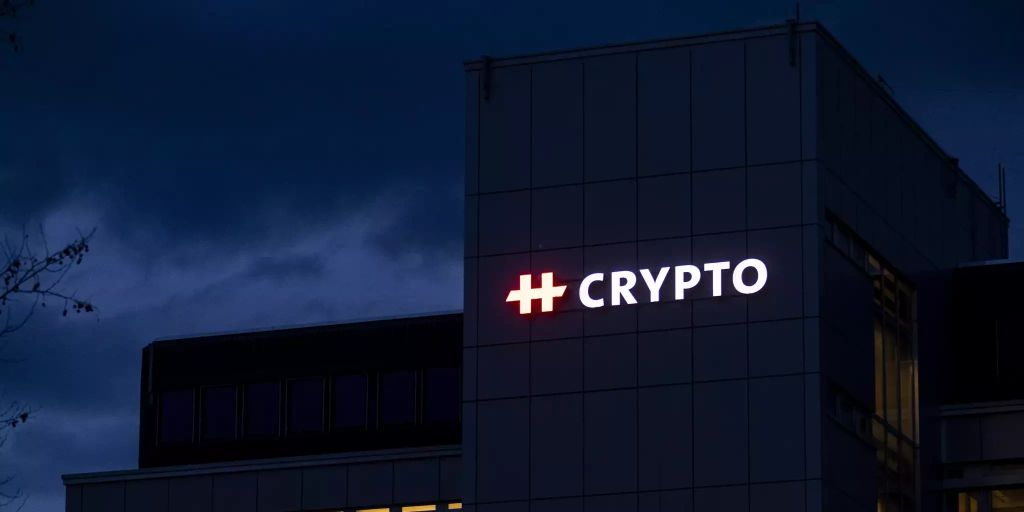
\includegraphics[width=\textwidth]{crypto-ag.jpg}
\end{frame}
\begin{frame}
	\frametitle{Which crypto?}
	\begin{itemize}
		\item Classical
		\item Modern
	\end{itemize}
	\note{
		So there are two categories of crypto.
		Classical is algorithms that could be used before computers were available,
		Modern is computer-assisted stuff.

		Right now the meta in CTFs leans more on modern crypto
		but we will also cover a bit of classical
	}
\end{frame}
\section{Theory}
\begin{frame}
	\frametitle{Prerequisites}
	\begin{itemize}
	\pause{}
\item discrete algebra
\item probability theory
	\end{itemize}
	\note{
		one bad thing with the crypto category is it can be less approachable because of all the math.
		OTOH it's also an opportunity to learn!

		We are going to cover some of the basics today
	}
\end{frame}
\begin{frame}
	\frametitle{Randomness}
	Let's play a game~!

	\note{
		game of guess the coin heads or tails
		lesson: assuming the coinflip is truly random, 50\% chance of winning at most
	}
	\pause{}
	\begin{itemize}
		\item I flip a coin
		\item You win if you guess the outcome
	\end{itemize}
	\begin{equation*}
		P(\text{win}) = \sfrac{1}{2}
	\end{equation*}
\end{frame}
\begin{frame}
	\frametitle{Pseudorandomness}
	Let's play a game~! (again)

	\pause{}
	\begin{itemize}
		\item The deterministic, polynomial time black box gets a private key of $k$ bits
		\item For any input, the blackbox returns 0 or 1 with equal probability
		\item You are also polynomial time in $O(k)$
		\item You can flip coins
		\item You win if you guess the output
	\end{itemize}
	\note{
		Here's this black box. (show debit card) We know it runs a deterministic algorithm, but there's also a secret key in it that we can't pull out.
		The goal is still to guess heads or tails. Also, we are computationally bounded to polynomial time in the length of the key. Can you do better than 50\%?
	}
	\pause{}
	\begin{equation*}
	P(\text{win at pseudorandom coin game}) \ge \sfrac{1}{2} + 2^k
	\end{equation*}
\end{frame}
\begin{frame}
	\frametitle{Why play games?}

	\begin{description}
		\item[Game] setup with win conditions and rules
		\item[Adversary] PPT algorithm that tries to win the game
		\item[PRF] pseudorandom function, blackbox from game \#2
	\end{description}
	\note{with games, we can formalize the security properties of constructs}
\end{frame}
\begin{frame}
	\frametitle{Message Authentication Codes}
	\begin{itemize}
		\item You leave data laying around unsupervised
		\item You want to know if anyone modifies it
		\item Compute a PRF on the data and append it
		\item Later, recompute the PRF and see if it matches the MAC
	\end{itemize}
\end{frame}
\begin{frame}
	\frametitle{pseudorandom permutation}
	\begin{description}
		\item[PRF] $f: {\{0,1\}}^k \rightarrow {\{0,1\}}^* \rightarrow {\{0,1\}}^l$
		\item[PRP] $p:  {\{0,1\}}^k \rightarrow {\{0,1\}}^l \rightarrow {\{0,1\}}^l$, $p^{-1}$ exists
	\end{description}
	Supports a simplistic encryption scheme: 
	\begin{itemize}
		\item encrypt with $p$
		\item decrypt with $p^{-1}$
		\item keep your key secret!
	\end{itemize}
	\note{
		pseudorandom permutations must be reversible by definition,
		so the codomain has to be the same as the domain.
		This is a basic building block for encryption.
		We'll see the pitfalls with that, but we have an interesting intuition there.
	}
\end{frame}
\begin{frame}
	\frametitle{public-key cryptography}
	\begin{itemize}
		\item symmetric primitives have one type of key.
		\item public-key encryption primitives have two different key.
		\item signing key and verifying key (MAC $\rightarrow$ digital signature)
		\item encryption key and decryption key
	\end{itemize}
	\note{
		again the simplified idea is you can publish your encryption key, and people can send you messages.
	}
\end{frame}
	\section{Practice}
\begin{frame}
	\frametitle{Cryptographic Hash functions}
	\begin{itemize}
		\item PRF but the key is public
		\item MD5, SHA-1, SHA-2 are insecure as MACs
		\item SHA-3 and Blake are like PRFs in practice
	\end{itemize}
\end{frame}
\begin{frame}
	\frametitle{Block ciphers}
	\begin{itemize}
		\item modelled after PRPs
		\item DES (bad), Blowfish, Rijndael/AES
		\item can build encryption systems using them
	\end{itemize}
\end{frame}
\begin{frame}
	\frametitle{Block cipher mode: Electronic code book}
	apply the same PRP to every block
\end{frame}
\begin{frame}
	\frametitle{Block cipher mode: Electronic code book}
	\begin{center}
		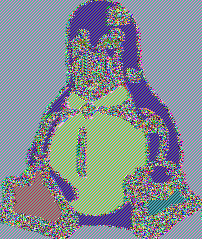
\includegraphics[height=0.8\textheight]{Tux_ECB.png}
	\end{center}
\end{frame}
\begin{frame}
	\frametitle{Block cipher mode}
	We want different outputs even if two input blocks are the same!
	\note{
		there are some simple ideas and some more complicated ones, let's look at some simple ideas
		anyone?
		(you're allowed to use xor)
	}
\end{frame}
\begin{frame}
	\frametitle{Cipher Block Chaining Mode}
	\begin{itemize}
		\item pick a per-message, non-secret initialization vector IV
		\item split plaintext in blocks
		\item pad the last block
		\item $CT_0 = Enc(IV \oplus PT_0)$
		\item $CT_1 = Enc(CT_0 \oplus PT_1)$
		\item \ldots
	\end{itemize}
\end{frame}
\begin{frame}
	\frametitle{Cipher Feedback Mode}
	\begin{itemize}
		\item pick a per-message, non-secret initialization vector IV
		\item compute a keystream $Enc(IV)$, $Enc(Enc(IV))$, etc.
		\item xor keystream with plaintext to get ciphertext
	\end{itemize}
\end{frame}
\begin{frame}
	\frametitle{what have we done? Stream cipher}
	\begin{itemize}
		\item generate a long, single-use, pseudorandom keystream
		\item xor with plaintext
		\item decryption is the same as encryption
		\item Example: Chacha20 and variants, RC4 (broken)
	\end{itemize}
\end{frame}
\section{Challenge methodology}
\begin{frame}
	\frametitle{The CTF cheatsheet}
	\pause{}
	\begin{center}
		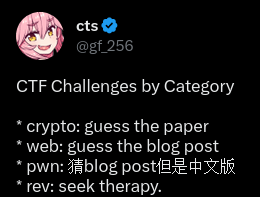
\includegraphics[height=0.8\textheight]{ctf_cheat_sheet.png}
	\end{center}
	\note{
		So the cheatsheet tells us to ``guess the paper''.
		There's a research paper out there that this chall is based on.
		How do we find papers?

		Second thing is knowing how to search.
		Most of the time there's something obscure for you to learn.
	}
\end{frame}
\begin{frame}
	\frametitle{Preprints}
	\begin{center}
		
\includegraphics[width=.4\textwidth]{iacrlogo.png}

	\url{https://eprint.iacr.org/}
	\end{center}
\end{frame}
\begin{frame}
	\frametitle{Preprints}
	\begin{center}
		
\includegraphics[width=.5\textwidth]{arxiv-logo.png}

		\url{https://arxiv.org/}
	\end{center}
	\note{
		There's a long tradition of Open Access in cryptology.
		This means that the vast majority of researchers will publish their papers online free-of-charge.
		(That's what makes it possible to do CTF at all)

		crypto eprints, specialized
		ArXiv, mathematics
	}
\end{frame}
\begin{frame}
	\frametitle{Abstraction levels}
	\emph{Program to an interface, not to an implementation}
	\note{
		Going back to levels of abstraction.
		There's a saying in software engineering.

		This is also the case in cryptography.

		Is the author re-implementing a primitive explicitly?
		Probably done on purpose.
		If they are using a well-known library then the issue is probably with interactions.

		For the longest time I thought elliptic curve formulas were confusing.
		Instead of bothering to study them more,
		I just took it for granted that they worked as an Abelian group and that the discrete logarithm was hard.
		And in a lot of cases that's all you need.
		Occasionally there are challs with broken elliptic curves or something,
		so I just left them for soemone else who's more advanced or more specialized.
	}
\end{frame}
\begin{frame}
	\frametitle{Tools of the trade: Cyberchef}
	\begin{center}
		\biglink{https://cyberchef.org/}
	\end{center}
	\note{
		First tool: cyberchef
		It's a toolbox that runs in your browser and can do various transformations on pieces of data.
		Let's check it out a bit.
		point out entropy, magic, modern ciphers, classical ciphers, filetype detection
		of course you can also do all of this on the terminal if you prefer
	}
\end{frame}
\begin{frame}
	\frametitle{Tools of the trade: Python 3}
Python has super\texttt{pow}ers
	\note{
		Python 3 is the most common language for both challs and solvescripts.
		The reason: with just the built-in stuff you already have modular exponentiation for arbitrarily big numbers
		Also the usual bitwise operations, standard hashes, etc.
		To prove this, here's a toy implementation of DSA signature generation.
	}
\end{frame}
\begin{frame}[fragile]
	\inputminted[]{python}{dsa_sign.py}
	\note{
		don't use this for serious stuff, it's just to show that it's here
		we're not done with python: let's talk about the libraries
	}
\end{frame}
\begin{frame}
	\frametitle{Tools of the trade: Python libs}
	\begin{itemize}
\item \texttt{pwntools}
\item \texttt{PyCryptoDome}
\item \texttt{fastecdsa}
\item Extra stuff from PyPI\@: \texttt{passlib}, \texttt{pgpy}, \texttt{blspy}, \texttt{web3} etc.
	\end{itemize}

	\note{

		You will want pwntools to talk with any remotes.
		You already know it, no need to look any further.

		PyCryptoDome has a lot of low-level crypto primitive and serialization formats.
		Get it too, it's free!

		If you need elliptic curve math, fastecdsa is your friend

		And if you need to go beyond that, PyPI has almost everything so search
	}


\end{frame}
\begin{frame}
	\frametitle{Tools of the trade: Sage}
	\note{
		The last tool is SageMath. It's a sofware system for mathematicians.
		In more esoterc challenges you might encounter it.

		There's this language that's overlaid on top of Python 3 but it's different in subtle ways
		I personally don't really like it because there are a lot of weird footguns lying around but you might still need it.
	}
\end{frame}
\begin{frame}
	\frametitle{Cryptohack docker}
	\begin{center}

		\biglink{https://github.com/cryptohack/cryptohack-docker}
	\end{center}
	\note{This is the CryptoHack docker container which has sage in it and heavily inspired ours.}
\end{frame}
\begin{frame}
	\begin{itemize}
		\item play
		\item read writeups
		\item follow crypto stuff
	\end{itemize}
	\note{
		play CTFs with us, play cryptohack, play imaginary.
		Then read writeups.
		Other thing you can do is join cryptography communities on your favorite social media.
		You can get exposed to interesting stuff. And a lot of drama. With a side order of interesting stuff.
	}
\end{frame}
\begin{frame}
	\frametitle{GIVE ME FLAGS}
	\begin{itemize}
		\item happens on the Discord
		\item more bits = harder
	\end{itemize}
	\note{
		I know I'm boring and some of you have been listening to boring nerds talk about crypto for way too long, so it's time to roll
	}
\end{frame}
\begin{frame}
	\begin{center}
		\biglink{https://discord.gg/VEtQUytz}
	\end{center}
\end{frame}
\end{document}
